\documentclass[border=7pt]{standalone}
\usepackage{fontspec,unicode-math}
\setmainfont{Noto Serif}
\setmathfont{STIXTwoMath-Regular.otf}
\usepackage{tikz}
\usetikzlibrary{arrows.meta,calc,patterns,decorations.pathreplacing,decorations.markings}
\tikzset{
  structure/.style={black,line width=.78pt,line join=round,line cap=round},
  potential/.style={black,line width=1.1pt,line join=round,line cap=round},
  level/.style={black,line width=1.04pt,line cap=butt},
  thinlevel/.style={black,line width=.66pt,line cap=butt},
  ax/.style={black,line width=.60pt,-{Latex[length=2mm,width=1.2mm]}},
  transition/.style={black,line width=.72pt,-{Latex[length=2mm,width=1.16mm]},shorten >=2pt,shorten <=2pt},
  dim/.style={black,line width=.66pt,{Latex[length=1.8mm,width=1mm]}-{Latex[length=1.8mm,width=1mm]}},
  annot/.style={font=\fontsize{11}{13}\selectfont,inner sep=1.6pt},
  panel/.style={font=\fontsize{13}{16}\selectfont\itshape,inner sep=1pt}
}
\pagestyle{empty}
\begin{document}
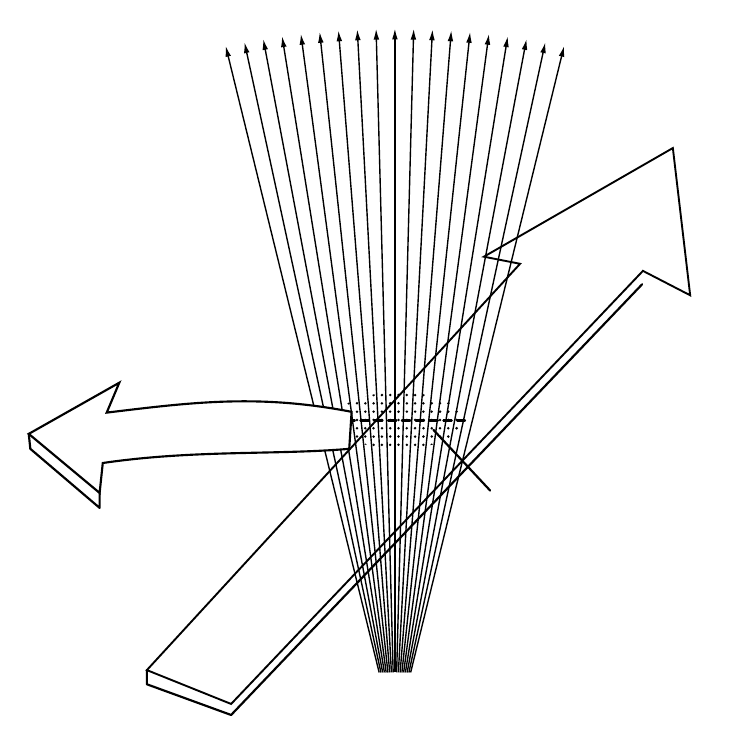
\begin{tikzpicture}[x=1cm,y=1cm]
% Physical basis: atom +z, light +y, ion extraction -x. Dot products == 0.
% Oblique 2D projection of the three perpendicular laboratory directions.
\coordinate (O) at (5.25,3.32);
\coordinate (zlow) at (5.00,0.18);
% Laser broad hollow arrow enters from near-left/bottom and proceeds to right/back.
\filldraw[fill=white,draw=black,line width=.68pt]
 (2.05,.15) -- (6.79,5.31) -- (6.33,5.40)
 -- (8.73,6.78) -- (8.95,4.91) -- (8.35,5.22)
 -- (3.12,-.28) -- cycle;
\draw[structure] (2.05,.15)--(2.05,-.03)--(3.12,-.42)--(8.34,5.05);
% Actual atom beam: 19 rays diverging from a narrow lower aperture.
\foreach \i in {0,...,18} {
 \pgfmathsetmacro{\u}{(\i-9)/9}
 \pgfmathsetmacro{\xstart}{5.20+0.20*\u}
 \pgfmathsetmacro{\xend}{5.20+2.15*\u}
 \pgfmathsetmacro{\yend}{8.30-0.22*\u*\u}
 \draw[black,line width=.50pt,-{Latex[length=1.4mm,width=.72mm]}]
 (\xstart,.12)--(\xend,\yend);
}
% Ionization volume: intersection, not a free fourth beam.
\fill[pattern=dots,pattern color=black] (O) ellipse (.82 and .36);
\draw[structure,densely dashed] (4.41,3.32)--(6.09,3.32);
% Left-moving ion beam originates in the dotted overlap; arrow is not perspective edge.
\filldraw[fill=white,draw=black,line width=.77pt]
 (4.65,3.43) .. controls (3.46,3.66) and (2.62,3.55) .. (1.54,3.42)
 --(1.70,3.80)--(.55,3.15)--(1.45,2.40)--(1.49,2.78)
 .. controls (2.65,2.95) and (3.68,2.88) .. (4.62,2.96) --cycle;
\draw[structure] (.55,3.15)--(.57,2.96)--(1.45,2.21)--(1.45,2.40);
\node[annot,anchor=west] at (7.28,7.70) {Атомный пучок};
\node[annot,anchor=west] at (7.19,7.14) {Лазерное излучение};
\node[annot,anchor=east] at (1.76,4.14) {Ионы};
\node[annot,anchor=west] (lbl) at (6.41,2.43) {Область ионизации};
\draw[structure] (lbl.west)--(5.69,3.20);
\end{tikzpicture}
\end{document}
